\section{PowderN: A general powder sample}
\index{Samples!Powder, multiple diffraction line}
\index{Diffraction}
\index{Sample environments}
\index{Concentric components}
\label{powder}

\section{PowderN: A general powder sample}
\index{Samples!Powder, multiple diffraction line}
\index{Diffraction}
\index{Sample environments}
\index{Concentric components}
\label{powder}

\component{Powder\_N}{System}{$radius$, $thickness$, $h$, $xwidth$, $yheight$, $zdepth$, $\sigma_{\rm abs}$,
  $\sigma_{\rm inc}$, $Vc$, $f_{\rm pack}$, reflections, format, DW, concentic, and more}{}{}

The powder diffraction component {\bf PowderN} models a powder sample
with background coming only from incoherent scattering and no
multiple scattering. At the users choice, a given percentage of the incoming
events may be transmitted (attenuated) to model the direct beam. The component can also
assume \emph{concentric} shape, i.e. be used for describing sample environment (cryostat,
sample container etc.). 

The description of the powder comes from a file in one of the standard output formats LAZY, FULLPROF, or CRYSTALLOGRAPHICA.

A usage example of this component can be found in the \\
\verb+Neutron site/Tutorial/templateDIFF+ instrument from the \verb+mcgui+.

\subsection{Files formats: powder structures}

Data files of type \verb'lau' and \verb'laz' in the \MCS distribution data directory are self-documented in their header. A list of common powder definition files is available in Table \ref{t:powders-data} (page \pageref{t:powders-data}). They do not need any additional parameters to be used, as in the example:
\begin{lstlisting}
  PowderN(<geometry parameters>, filename="Al.laz")
\end{lstlisting}
Other column-based file formats may also be imported e.g. with parameters such as:
\begin{lstlisting}
  format=Crystallographica
  format=Fullprof
  format={1,2,3,4,0,0,0,0}
\end{lstlisting}
In the latter case, the indices define order of columns parameters
multiplicity, lattice spacing, $F^2$, Debye-Waller factor and intrinsic line width.

The column signification may as well explicitely be set in the data file header using any of the lines:
\begin{lstlisting}
  #column_j     <index of the multiplicity 'j' column>
  #column_d     <index of the d-spacing 'd' column>
  #column_F2    <index of the squared str. factor '|F|^2' column [b]>
  #column_F     <index of the structure factor norm '|F|' column>
  #column_DW    <index of the Debye-Waller factor 'DW' column>
  #column_Dd    <index of the relative line width Delta_d/d 'Dd' column>
  #column_inv2d <index of the 1/2d=sin(theta)/lambda 'inv2d' column>
  #column_q     <index of the scattering wavevector 'q' column>
\end{lstlisting}

Other component parameters may as well be specified in the data file
header with lines e.g.:
\begin{lstlisting}
  #V_rho        <value of atom number density [at/Angs^3]>
  #Vc           <value of unit cell volume Vc [Angs^3]>
  #sigma_abs    <value of Absorption cross section [barns]>
  #sigma_inc    <value of Incoherent cross section [barns]>
  #Debye_Waller <value of Debye-Waller factor DW>
  #Delta_d/d    <value of Detla_d/d width for all lines>
  #density      <value of material density [g/cm^3]>
  #weight       <value of material molar weight [g/mol]>
  #nb_atoms     <value of number of atoms per unit cell>
\end{lstlisting}

Further details on file formats are available in the \verb+mcdoc+ page
of the component.

\subsection{Geometry, physical properties, concentricity}
The sample has the shape of a solid cylinder, radius $r$ and height $h$ or a box-shaped
sample of size $xwidth$ x $yheight$ x $zdepth$. At the users choice, an inner 'hollow' can be
specified using the parameter $thickness$. 


As the Isotropic\_Sqw component~\ref{s:isotropic-sqw}, PowderN assumes \emph{concentric} shape, i.e.
can contain other components inside the inner hollow. To allow this, two almost identical copies
of the PowderN components must be set up \emph{around} the internal component(s), for example:


\begin{lstlisting}
COMPONENT Cryo = PowderN(reflections="Al.laz", radius = 0.01, thickness = 0.001,
                          concentric = 1)
AT (0,0,0) RELATIVE Somewhere

COMPONENT Sample = some_other_component(with geometry FULLY enclosed in the hollow)
AT (0,0,0) RELATIVE Somewhere

COMPONENT Cryo2 = COPY(Cryo)(concentric = 0)
AT (0,0,0) RELATIVE Somewhere
\end{lstlisting}

As outlined, the first instance of PowderN \emph{must} have \verb+concentric = 1+ and the instance \emph{must}
have \verb+concentric = 0+. Furthermore, the component(s) inside the hollow \emph{must} have a geometry which can
be fully contained inside the hollow.


In addition to the coherent scattering specified in the \verb+reflections+ file, absorption- and incoherent 
cross sections can be given using the input parameters $\sigma_c^a$ and $\sigma_i^s$.


The Bragg scattering from the powder,
$\sigma_c^s$ is calculated from the input file, with the parameters
$Q$, $|F(Q)|^2$, and $j$ for the scattering vector, structure factor, and
multiplicity, respectively. The volume of the unit cell is denoted $Vc$,
while the sample packing factor is $f_{\rm pack}$.


%Further, the incoherent scattering is only taken into account
%by the attenuation of the beam, given by (\ref{e:attenu})
%and $\sigma_c^a$.
%The incoherently scattered neutrons are not
%propagated through to the detector, but rather not generated at all.

Focusing is performed by only scattering into one angular
interval, $d\phi$ of the Debye-Scherrer circle. The center of this
interval is located at the point where the Debye-Scherrer circle
intersects the half-plane defined by the initial velocity, ${\bf v}_{\rm i}$,
and a user-specified vector, {\bf f}.

%The input parameters for this component are
%
%\begin{lstlisting}\begin{tabular}{ccl}
%$r$ & m & Radius of cylinder \\
%$h$ & m & Height of cylinder \\
%$\sigma_c^a$ & fm$^2$ & Absorption cross section per unit cell (at 2200 m/s) \\
%$\sigma_{i,c}^s$ & (fm)$^2$ & Incoherent scattering cross section per unit cell \\
%$\rho'/\rho$ & 1 & Packing factor \\
%$V_c$ & \AA$^3$ & Volume of unit cell \\
%${\bf Q}$ & \AA$^{-1}$ & The reciprocal lattice vector under consideration \\
%$|F({\bf Q}_j)|^2$ & (fm)$^2$ &
% Structure factor \\
%$j$ & 1 & Multiplicity of reflection \\
%$\exp(-2W)$ & 1 & Debye-Waller factor \\
%$d\phi$ & deg & Angular interval of focusing \\
%$f_x$ & m & \\
%$f_y$ & m & Focusing vector\\
%$f_z$ & m & \\
%\end{tabular}\end{lstlisting}

\subsection{Powder scattering}
An ideal powder sample consists of many small
crystallites, although each crystallite is sufficiently
large not to cause measurable size broadening.
The orientation of the crystallites is evenly distributed,
and there is thus always a large number of
crystallites oriented to fulfill the Bragg condition
\begin{equation}   \label{Bragg}
n \lambda = 2 d \sin \theta ,
\end{equation}
where $n$ is the order of the scattering (an integer), $\lambda$
is the neutron wavelength, $d$ is the lattice spacing of the sample,
and $2 \theta$ is the scattering angle, see figure \ref{coneFig}.
As all crystal orientations
are realised in a powder sample, the neutrons are scattered within a
{\em Debye-Scherrer cone} of opening angle $4 \theta$ \cite{bacon}.

\begin{figure}
  \begin{center}
    \psfrag{2theta}[c][c]{$2\theta$}
    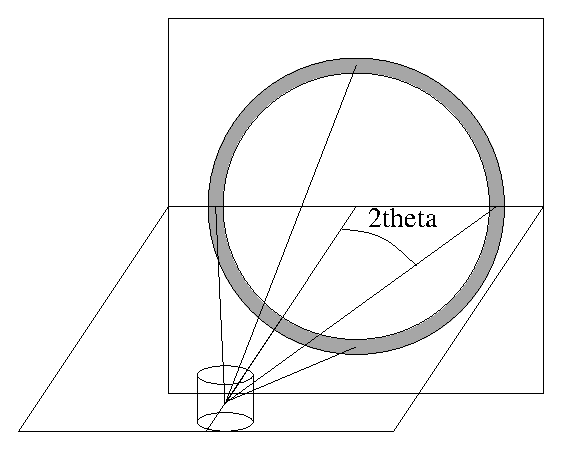
\includegraphics[width=0.6\textwidth]{figures/powder}
  \end{center}
\caption{The scattering geometry of a powder sample showing part of the
Debye-Scherrer cone (solid lines) and the Debye-Scherrer circle (grey).}
\label{coneFig}
\end{figure}

Equation (\ref{Bragg}) may be cast into the form
\begin{equation}
|{\bf Q}| = 2 |{\bf k}| \sin \theta ,
\end{equation}
where {\bf Q} is a vector of the reciprocal lattice, and {\bf k} is
the wave vector of the neutron. It is seen that only
reciprocal vectors fulfilling $|{\bf Q}| < 2 |{\bf k}|$
contribute to the scattering.
For a complete treatment of the powder sample, one needs to take
into account all these {\bf Q}-values, since each of them contribute
to the attenuation.

The strength of the Bragg reflections is given by their structure factors
\begin{equation}
 \left| \sum_j b_j \exp({\bf R}_j \cdot {\bf Q}) \right|^2 ,
\end{equation}
where the sum runs over all atoms in one unit cell. This structure factor is
non-zero only when $Q$ equals a reciprocal lattice vector.

The textbook expression for the scattering cross section
corresponding to one Debye-Scherrer cone reads \cite[ch.3.6]{squires}, with $V=N V_0$ being the total sample volume:
\begin{equation}
\sigma_{\rm cone}
  = \frac{V}{V_0^2} \frac{\lambda^3}{4 \sin \theta} \sum_Q |F(Q)|^2 .
\end{equation}
For our purpose, this expression should be changed slightly.
Firstly, the sum over structure factors for a particular $Q$ is replaced
by the sum over essentially different reflections multiplied by their
multiplicity, $j$. Then, a finite packing factor, $f$, is defined for the powder,
and finally, the Debye-Waller factor is multiplied on the elastic cross section
to take lattice vibrations into account (no inelastic background is simulated,
however). We then reach
\begin{eqnarray}
\sigma_{\rm cone, Q}
 & = & j_Q f \exp(-2W) \frac{V}{V_0^2} \frac{\lambda^3}{4 \sin \theta} |F(Q)|^2 \\
 & = & f \exp(-2W) \frac{N}{V_0} \frac{4\pi^3}{k^2} \frac{j_Q |F(Q)|^2}{Q}
\end{eqnarray}
in the thin sample approximation. For samples of finite thickness, the
beam is being attenuated by the attenuation coefficient
\begin{equation}
\label{e:attenu}
\mu_{\rm Q} = \sigma_{\rm cone,Q} / V .
\end{equation}
For calibration it may be useful to consider the total intensity
scattered into a detector of effective height $h$, covering only
one reflection \cite[ch.3.6]{squires}.
A cut though the Debye-Scherrer cone perpendicular to its axis
is a circle. At the distance $r$ from the sample, the radius of this
circle is $r \sin(2\theta)$. Thus, the detector (in a small angle
approximation) counts a fraction $h / (2 \pi r \sin(2 \theta))$
of the scattered neutrons, giving a resulting count intensity:
\begin{equation}
I = \Psi \sigma_{\rm cone,Q} \frac{h}{2 \pi r \sin(2\theta)} ,
\end{equation}
where $\Psi$ is the flux at the sample position.

For clarity we repeat the meaning and unit of the symbols:
%
\begin{lstlisting}
\begin{tabular}{ccl}
$\Psi$ & s$^{-1}$m$^{-2}$ & Incoming intensity of neutrons \\
$I$    & s$^{-1}$ & Detected intensity of neutrons \\
$h$    & m        & Height of detector \\
$r$    & m        & Distance from sample to detector \\
$f$    & 1        & Packing factor of the powder \\
$j$    & 1        & Multiplicity of the reflection \\
$V_0$  & m$^{3}$  & Volume of unit cell\\
$|F({\bf Q})|^2$ & m$^2$  & Structure factor \\
$\exp(-2W)$ & 1  & Debye-Waller factor \\
$\mu_{\rm Q}$ & m$^{-1}$ & Linear attenuation factor due to scattering from
one powder line. \\
\end{tabular}
\end{lstlisting}
%
%Often, one defines the {\em scattering power} as
%\begin{equation}
%Q \equiv N^2 \frac{|F({\bf Q})|^2 \lambda^3}{V \sin(2\theta)}
% = N_c^2 V \frac{\rho'}{\rho} \frac{|F({\bf Q})|^2 \lambda^3}{\sin(2\theta)} ,
%\end{equation}
%where $N$ is the number of unit cells.

A powder sample will in general have several allowed reflections
${\bf Q}_j$, which will all contribute to the attenuation.
These reflections will have different values of
$|F({\bf Q}_j)|^2$ (and hence of $Q_j$), $j_j$, $\exp(-2W_j)$,
and $\theta_j$.
The total attenuation through the sample due to scattering is given by
$\mu^s = \mu_{\rm inc}^s + \sum_j \mu^s_j $,
where $\mu_{\rm inc}^s$ represents the incoherent scattering.

\subsection{Algorithm}
The algorithm of {\bf PowderN} can be summarized as
\begin{itemize}
\item Check if the neutron ray intersects the sample (otherwise ignore
the following).
\item Calculate the attenuation coefficients for scattering and absorption.
\item Perform Monte Carlo choices to determine the scattering position,
scattering type (coherent/incoherent), and the outgoing direction.
\item Perform the necessary weight factor transformation.
\end{itemize}

%\subsection{Calculating the weight factor}

%\component{Powder\_N}{System}{$radius$, $thickness$, $h$, $xwidth$, $yheight$, $zdepth$, $\sigma_\mathrm{abs}$,
%  $\sigma_\mathrm{inc}$, $Vc$, $f_\mathrm{pack}$, reflections, format, DW, concentic, and more}{}{}

The powder diffraction component \textbf{PowderN} models a powder sample
with background coming only from incoherent scattering and no
multiple scattering. At the users choice, a given percentage of the incoming
events may be transmitted (attenuated) to model the direct beam. The component can also
assume \emph{concentric} shape, i.e. be used for describing sample environment (cryostat,
sample container etc.). 

The description of the powder comes from a file in one of the standard output formats LAZY, FULLPROF, or CRYSTALLOGRAPHICA.

%A usage example of this component can be found in the \\
%\verb+x-ray site/Tutorial/templateDIFF+ instrument from the \verb+mcgui+.

\subsection{Files formats: powder structures}

Data files of type \verb'lau' and \verb'laz' in the \MCX distribution data directory are self-documented in their header. 
%A list of common powder definition files is available in Table \ref{t:powders-data} (page \pageref{t:powders-data}). They do not need any additional parameters to be used, as in the example:
\begin{verbatim}
  PowderN(<geometry parameters>, filename="Al.laz")
\end{verbatim}
Other column-based file formats may also be imported e.g. with parameters such as:
\begin{verbatim}
  format=Crystallographica
  format=Fullprof
  format={1,2,3,4,0,0,0,0}
\end{verbatim}
In the latter case, the indices define order of columns parameters
multiplicity, lattice spacing, $F^2$, Debye-Waller factor and intrinsic line width.

The column signification may as well explicitely be set in the data file header using any of the lines:
\begin{verbatim}
  #column_j     <index of the multiplicity 'j' column>
  #column_d     <index of the d-spacing 'd' column>
  #column_F2    <index of the squared str. factor '|F|^2' column [b]>
  #column_F     <index of the structure factor norm '|F|' column>
  #column_DW    <index of the Debye-Waller factor 'DW' column>
  #column_Dd    <index of the relative line width Delta_d/d 'Dd' column>
  #column_inv2d <index of the 1/2d=sin(theta)/lambda 'inv2d' column>
  #column_q     <index of the scattering wavevector 'q' column>
\end{verbatim}

Other component parameters may as well be specified in the data file
header with lines e.g.:
\begin{verbatim}
  #V_rho        <value of atom number density [at/Angs^3]>
  #Vc           <value of unit cell volume Vc [Angs^3]>
  #sigma_abs    <value of Absorption cross section [barns]>
  #sigma_inc    <value of Incoherent cross section [barns]>
  #Debye_Waller <value of Debye-Waller factor DW>
  #Delta_d/d    <value of Detla_d/d width for all lines>
  #density      <value of material density [g/cm^3]>
  #weight       <value of material molar weight [g/mol]>
  #nb_atoms     <value of number of atoms per unit cell>
\end{verbatim}

Further details on file formats are available in the \texttt{mxdoc} page
of the component.

\subsection{Geometry, physical properties, concentricity}
The sample has the shape of a solid cylinder, radius $r$ and height $h$ or a box-shaped
sample of size $xwidth$ x $yheight$ x $zdepth$. At the users choice, an inner 'hollow' can be
specified using the parameter $thickness$. 


%As the Isotropic\_Sqw component~\ref{s:isotropic-sqw}, 
PowderN can assume a \emph{concentric} shape, i.e.
can contain other components inside the inner hollow. To allow this, two almost identical copies
of the PowderN components must be set up \emph{around} the internal component(s), for example:


\begin{verbatim}
COMPONENT Cryo = PowderN(reflections="Al.laz", radius = 0.01, thickness = 0.001,
                          concentric = 1)
AT (0,0,0) RELATIVE Somewhere

COMPONENT Sample = some_other_component(with geometry FULLY enclosed in the hollow)
AT (0,0,0) RELATIVE Somewhere

COMPONENT Cryo2 = COPY(Cryo)(concentric = 0)
AT (0,0,0) RELATIVE Somewhere
\end{verbatim}

As outlined, the first instance of PowderN \emph{must} have \texttt{concentric = 1} and the second instance \emph{must}
have \texttt{concentric = 0}. Furthermore, the component(s) inside the hollow \emph{must} have a geometry which can
be fully contained inside the hollow.


In addition to the coherent scattering specified in the \verb+reflections+ file, absorption- and incoherent 
cross sections can be given using the input parameters $\sigma_c^a$ and $\sigma_i^s$.


The Bragg scattering from the powder,
$\sigma_c^s$ is calculated from the input file, with the parameters
$Q$, $|F(Q)|^2$, and $j$ for the scattering vector, structure factor, and
multiplicity, respectively. The volume of the unit cell is denoted $Vc$,
while the sample packing factor is $f_\mathrm{pack}$.


%Further, the incoherent scattering is only taken into account
%by the attenuation of the beam, given by (\ref{e:attenu})
%and $\sigma_c^a$.
%The incoherently scattered x-rays are not
%propagated through to the detector, but rather not generated at all.

Focusing is performed by only scattering into one angular
interval, $d\phi$ of the Debye-Scherrer circle. The center of this
interval is located at the point where the Debye-Scherrer circle
intersects the half-plane defined by the initial velocity, $\boldsymbol{v}_\mathrm{i}$,
and a user-specified vector, $\boldsymbol{f}$.

%The input parameters for this component are
%
%\begin{quote}\begin{tabular}{ccl}
%$r$ & m & Radius of cylinder \\
%$h$ & m & Height of cylinder \\
%$\sigma_c^a$ & fm$^2$ & Absorption cross section per unit cell (at 2200 m/s) \\
%$\sigma_{i,c}^s$ & (fm)$^2$ & Incoherent scattering cross section per unit cell \\
%$\rho'/\rho$ & 1 & Packing factor \\
%$V_c$ & \AA$^3$ & Volume of unit cell \\
%$\boldsymbol{Q}$ & \AA$^{-1}$ & The reciprocal lattice vector under consideration \\
%$|F(\textbf{Q}_j)|^2$ & (fm)$^2$ &
% Structure factor \\
%$j$ & 1 & Multiplicity of reflection \\
%$\exp(-2W)$ & 1 & Debye-Waller factor \\
%$d\phi$ & deg & Angular interval of focusing \\
%$f_x$ & m & \\
%$f_y$ & m & Focusing vector\\
%$f_z$ & m & \\
%\end{tabular}\end{quote}

\subsection{Powder scattering}
An ideal powder sample consists of many small
crystallites, although each crystallite is sufficiently
large not to cause measurable size broadening.
The orientation of the crystallites is evenly distributed,
and there is thus always a large number of
crystallites oriented to fulfill the Bragg condition
\begin{equation}   \label{Bragg}
n \lambda = 2 d \sin \theta ,
\end{equation}
where $n$ is the order of the scattering (an integer), $\lambda$
is the x-ray wavelength, $d$ is the lattice spacing of the sample,
and $2 \theta$ is the scattering angle, see figure \ref{coneFig}.
As all crystal orientations
are realised in a powder sample, the x-rays are scattered within a
{\em Debye-Scherrer cone} of opening angle $4 \theta$ \cite{bacon}.

\begin{figure}
  \begin{center}
    \psfrag{2theta}[c][c]{$2\theta$}
    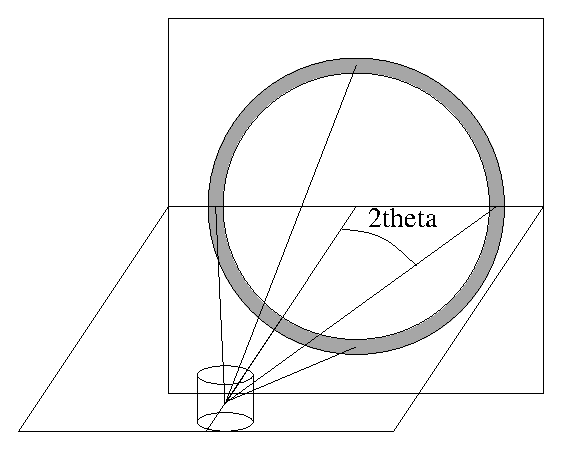
\includegraphics[width=0.6\textwidth]{figures/powder.eps}
  \end{center}
\caption{The scattering geometry of a powder sample showing part of the
Debye-Scherrer cone (solid lines) and the Debye-Scherrer circle (grey).}
\label{coneFig}
\end{figure}

Equation (\ref{Bragg}) may be cast into the form
\begin{equation}
|\boldsymbol{Q}| = 2 |\boldsymbol{k}| \sin \theta ,
\end{equation}
where \textbf{Q} is a vector of the reciprocal lattice, and \textbf{k} is
the wave vector of the x-ray. It is seen that only
reciprocal vectors fulfilling $|\boldsymbol{Q}| < 2 |\boldsymbol{k}|$
contribute to the scattering.
For a complete treatment of the powder sample, one needs to take
into account all these \textbf{Q}-values, since each of them contribute
to the attenuation.

The strength of the Bragg reflections is given by their structure factors
\begin{equation}
 \left| \sum_j b_j \exp(\boldsymbol{R}_j \cdot \boldsymbol{Q}) \right|^2 ,
\end{equation}
where the sum runs over all atoms in one unit cell. This structure factor is
non-zero only when $Q$ equals a reciprocal lattice vector.

The textbook expression for the scattering cross section
corresponding to one Debye-Scherrer cone reads \cite[ch.3.6]{squires}, with $V=N V_0$ being the total sample volume:
\begin{equation}
\sigma_\mathrm{cone}
  = \frac{V}{V_0^2} \frac{\lambda^3}{4 \sin \theta} \sum_Q |F(Q)|^2 .
\end{equation}
For our purpose, this expression should be changed slightly.
Firstly, the sum over structure factors for a particular $Q$ is replaced
by the sum over essentially different reflections multiplied by their
multiplicity, $j$. Then, a finite packing factor, $f$, is defined for the powder,
and finally, the Debye-Waller factor is multiplied on the elastic cross section
to take lattice vibrations into account (no inelastic background is simulated,
however). We then reach
\begin{eqnarray}
\sigma_\mathrm{cone, Q}
 & = & j_Q f \exp(-2W) \frac{V}{V_0^2} \frac{\lambda^3}{4 \sin \theta} |F(Q)|^2 \\
 & = & f \exp(-2W) \frac{N}{V_0} \frac{4\pi^3}{k^2} \frac{j_Q |F(Q)|^2}{Q}
\end{eqnarray}
in the thin sample approximation. For samples of finite thickness, the
beam is being attenuated by the attenuation coefficient
\begin{equation}
\label{e:attenu}
\mu_\mathrm{Q} = \sigma_\mathrm{cone,Q} / V .
\end{equation}
For calibration it may be useful to consider the total intensity
scattered into a detector of effective height $h$, covering only
one reflection \cite[ch.3.6]{squires}.
A cut though the Debye-Scherrer cone perpendicular to its axis
is a circle. At the distance $r$ from the sample, the radius of this
circle is $r \sin(2\theta)$. Thus, the detector (in a small angle
approximation) counts a fraction $h / (2 \pi r \sin(2 \theta))$
of the scattered x-rays, giving a resulting count intensity:
\begin{equation}
I = \Psi \sigma_\mathrm{cone,Q} \frac{h}{2 \pi r \sin(2\theta)} ,
\end{equation}
where $\Psi$ is the flux at the sample position.

For clarity we repeat the meaning and unit of the symbols:
%
\begin{quote}\begin{tabular}{ccl}
$\Psi$ & s$^{-1}$m$^{-2}$ & Incoming intensity of x-rays \\
$I$    & s$^{-1}$ & Detected intensity of x-rays \\
$h$    & m        & Height of detector \\
$r$    & m        & Distance from sample to detector \\
$f$    & 1        & Packing factor of the powder \\
$j$    & 1        & Multiplicity of the reflection \\
$V_0$  & m$^{3}$  & Volume of unit cell\\
$|F(\boldsymbol{Q})|^2$ & m$^2$  & Structure factor \\
$\exp(-2W)$ & 1  & Debye-Waller factor \\
$\mu_\mathrm{Q}$ & m$^{-1}$ & Linear attenuation factor due to scattering from
one powder line. \\
\end{tabular}\end{quote}
%
%Often, one defines the {\em scattering power} as
%\begin{equation}
%Q \equiv N^2 \frac{|F(\boldsymbol{Q})|^2 \lambda^3}{V \sin(2\theta)}
% = N_c^2 V \frac{\rho'}{\rho} \frac{|F(\boldsymbol{Q})|^2 \lambda^3}{\sin(2\theta)} ,
%\end{equation}
%where $N$ is the number of unit cells.

A powder sample will in general have several allowed reflections
$\boldsymbol{Q}_j$, which will all contribute to the attenuation.
These reflections will have different values of
$|F(\boldsymbol{Q}_j)|^2$ (and hence of $Q_j$), $j_j$, $\exp(-2W_j)$,
and $\theta_j$.
The total attenuation through the sample due to scattering is given by
$\mu^s = \mu_\mathrm{inc}^s + \sum_j \mu^s_j $,
where $\mu_\mathrm{inc}^s$ represents the incoherent scattering.

\subsection{Algorithm}
The algorithm of \textbf{PowderN} can be summarized as
\begin{itemize}
\item Check if the x-ray intersects the sample (otherwise ignore
the following).
\item Calculate the attenuation coefficients for scattering and absorption.
\item Perform Monte Carlo choices to determine the scattering position,
scattering type (coherent/incoherent), and the outgoing direction.
\item Perform the necessary weight factor transformation.
\end{itemize}

%\subsection{Calculating the weight factor}
